\documentclass{article}[18pt]
\usepackage{../../../../format}
\lhead{CSys}


\begin{document}
\begin{center}
\underline{\huge MIPS}
\end{center}
\section{Introduction}
MIPS - Microprocessor without Interlocked Pipeline Stages\\
\\
Underlying design principles:
\begin{itemize}
	\item Simplicity favours regularity
	\item Make the common case fast
	\item Smaller is faster
	\item Good design demands good compromises 
\end{itemize}
\section{32 Bit RISC Processor}
\begin{itemize}
	\item Around 80 instructions in the instruction set
	\item 32 general purpose registers \$r0 - \$r31
	\item \$r0 is special and always contains the value 0
	\item The MIPS processor has a super pipelined architecture - each instruction is broken down into a sequence of 'micro' instructions
\end{itemize}
\section{Design principles}
MIPS is a reduced instruction set computer (RISC), with a small number of simple instructions. Other architectures, such as intel's x86 are complex instruction set computers (CISC)


\begin{itemize}
	\item Simplicity favours regularity
	\begin{itemize}
		\item Consistent instruction format: same number of operands (two sources and one destination) is easier to encode and handle in hardware
	\end{itemize}
	\item Make the common use case fast
	\begin{itemize}
		\item MIPS includes only simple, commonly used instructions
		\item Hardware to decode and execute instructions can be simple, small and fast
		\item More complex instructions (that are less common) performed using multiple simple instructions
	\end{itemize}
	\item Smaller is faster
	\begin{itemize}
		\item MIPS includes only a small number of registers
		\begin{center}
			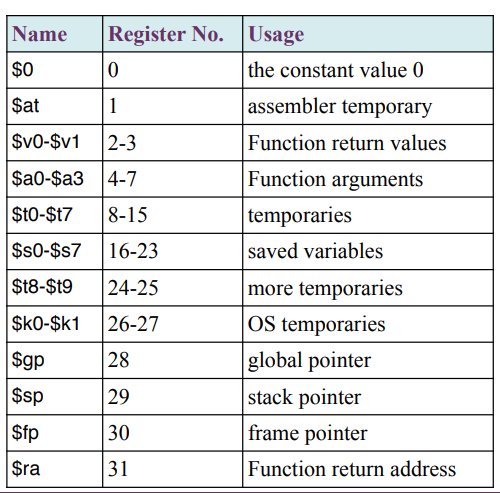
\includegraphics[scale=0.5]{register}
		\end{center}
	\end{itemize}
	\item Good design demands good compromises
	\begin{itemize}
		\item Multiple instruction formates allow flexibility, for example some use 3 operands, some 2
		\item Number of instruction formats kept small to adhere to design principles 1 and 3
		\item Other formats appear in assembler, but are transformed into machine code to fit with this format
	\end{itemize} 
\end{itemize}
\section{Instruction Types}
\subsection{R Type}
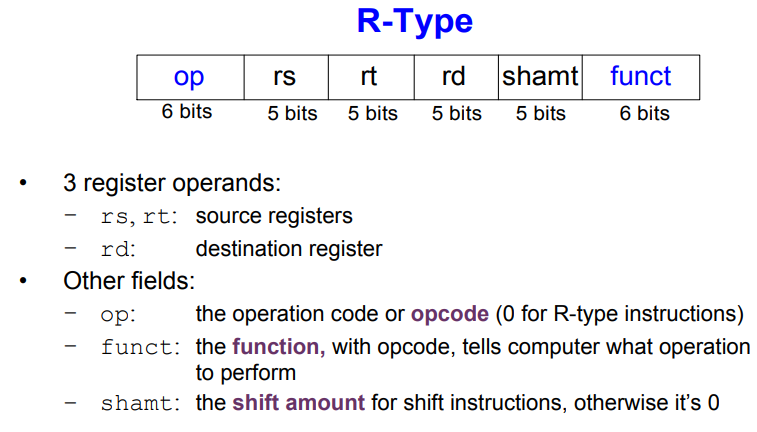
\includegraphics[scale=0.7]{R-Type}\\
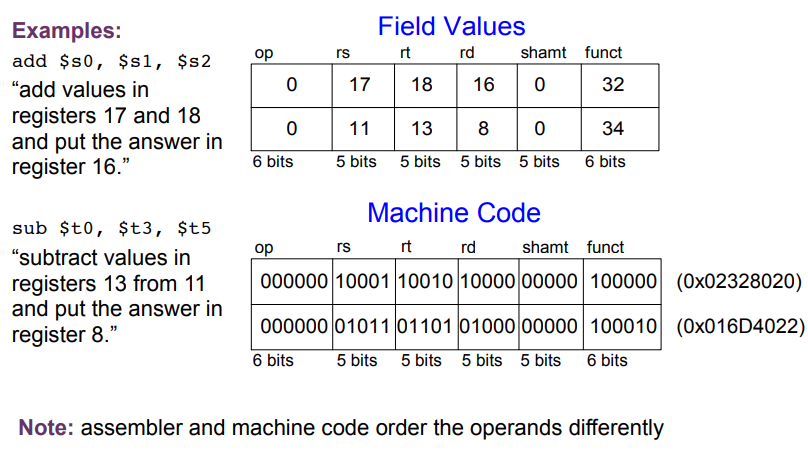
\includegraphics[scale=0.7]{R-Type1}\\
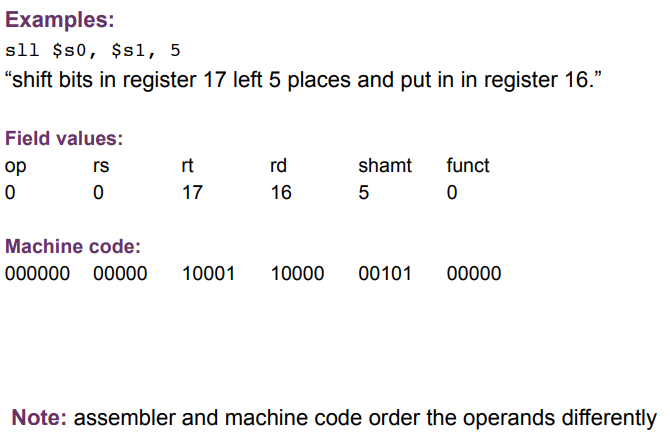
\includegraphics[scale=0.7]{R-Type2}
\subsection{I Type}
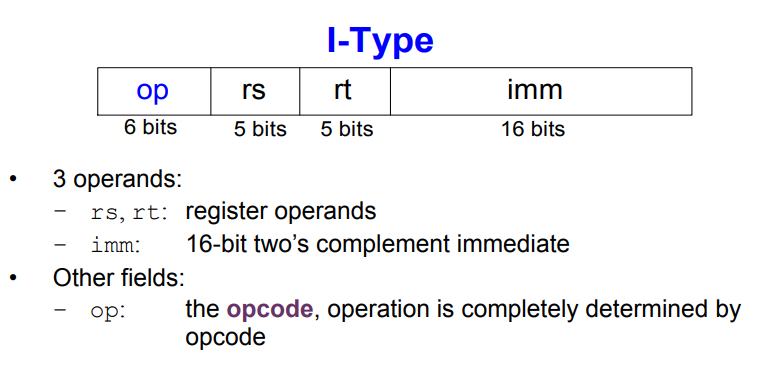
\includegraphics[scale=0.7]{I-Type}\\
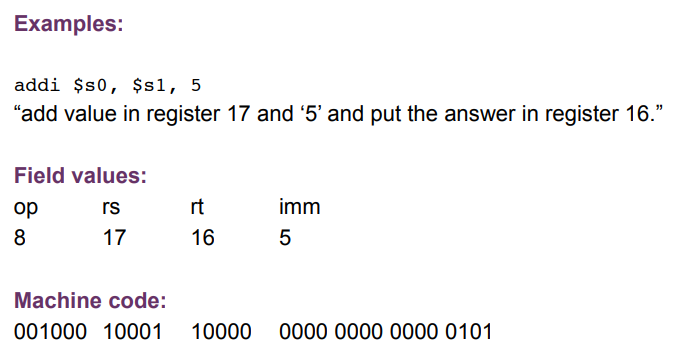
\includegraphics[scale=0.7]{I-Type1}\\
\subsection{J Type}
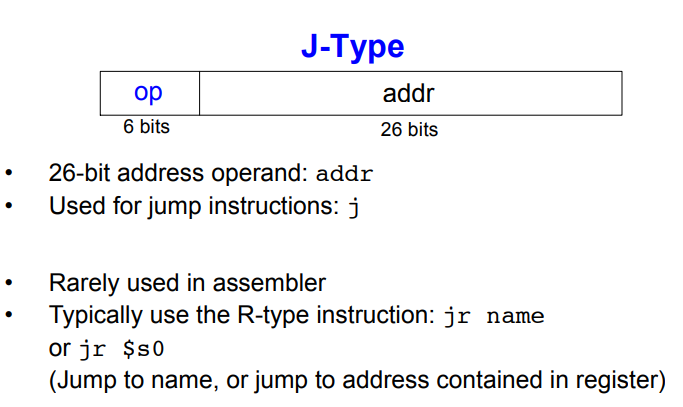
\includegraphics[scale=0.7]{J-Type}
\section{Addressing}
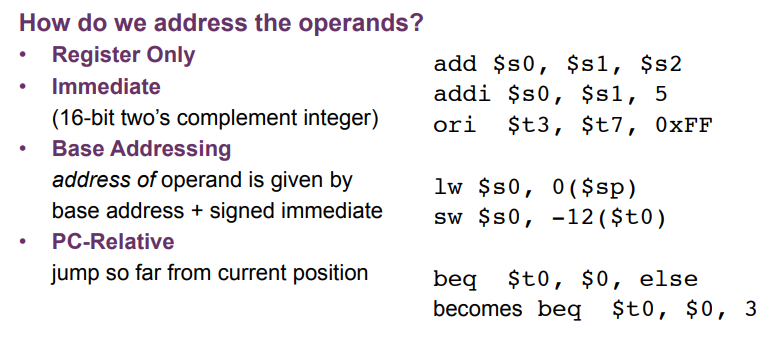
\includegraphics[scale=0.7]{Addressing}\\
There is the 3 at the end of the pc relative jump because it jumps 3 lines ahead in the program\\
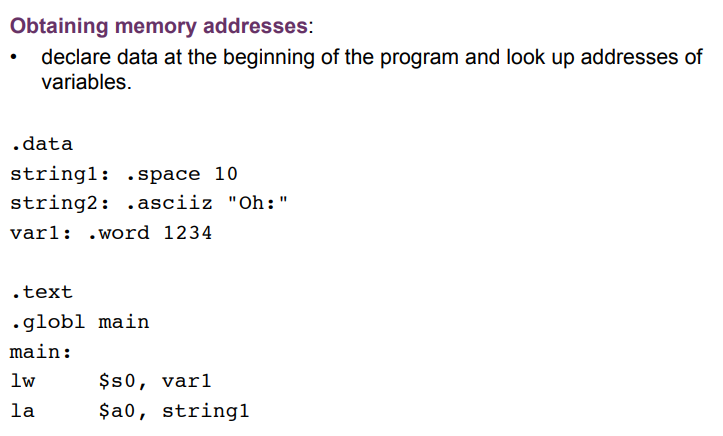
\includegraphics[scale=0.7]{Addressing1}
\section{Loading 32 Bit words}
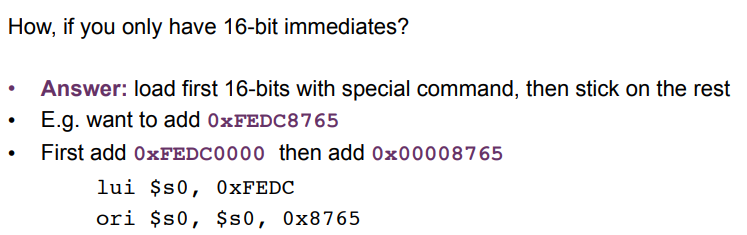
\includegraphics[scale=0.7]{32-Bit}\\
This loads half into the left half of the bits, and the other half into the right half
\section{OS Calls}
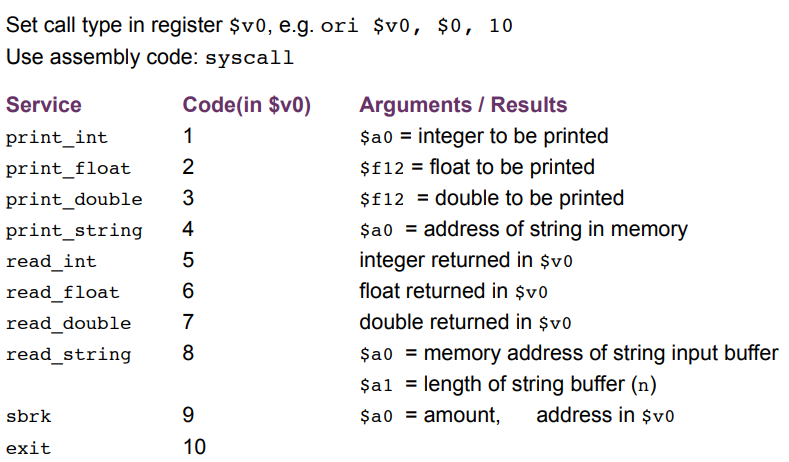
\includegraphics[scale=0.7]{OS-Call}
\section{Multiplication and Division}
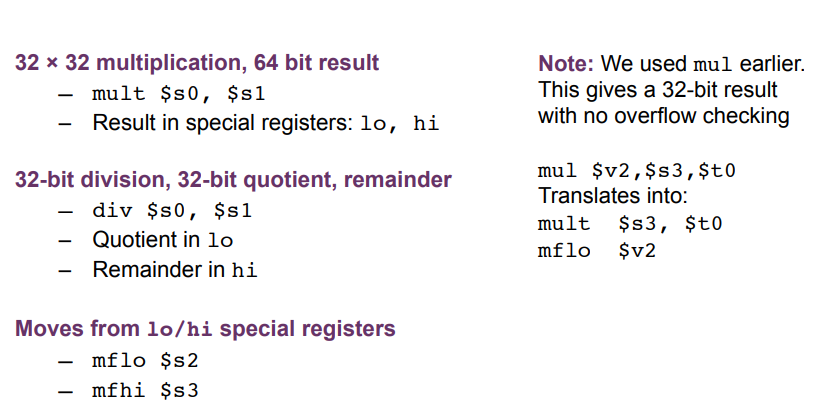
\includegraphics[scale=0.7]{Mult}
\section{MIPS Function Calls}
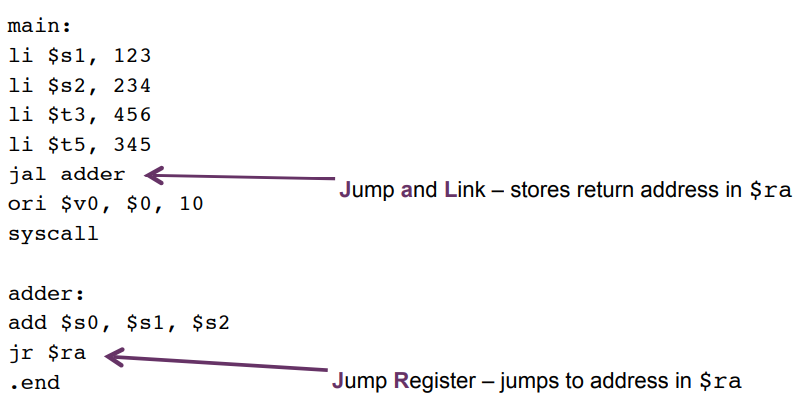
\includegraphics[scale=0.7]{Function}
\section{Conventions}
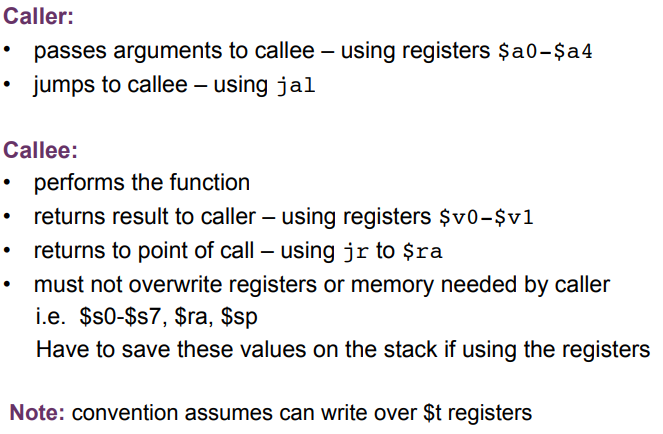
\includegraphics[scale=0.7]{Conventions}\\
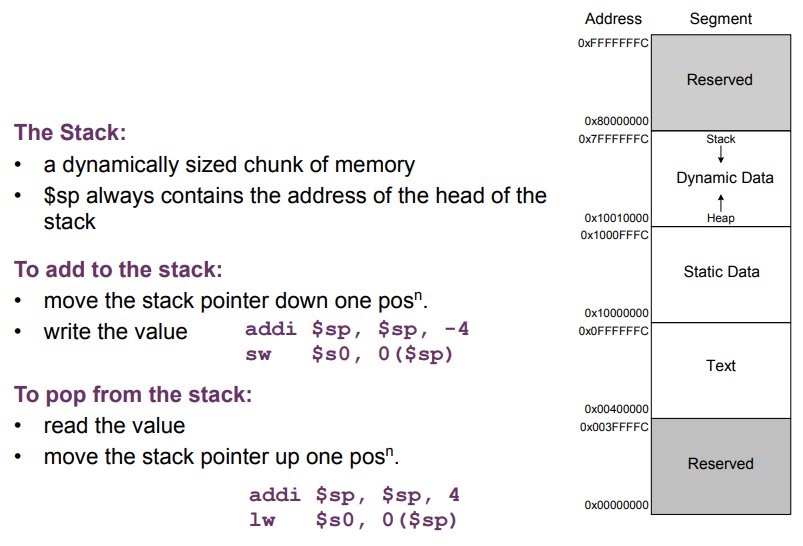
\includegraphics[scale=0.7]{Conventions1}\\
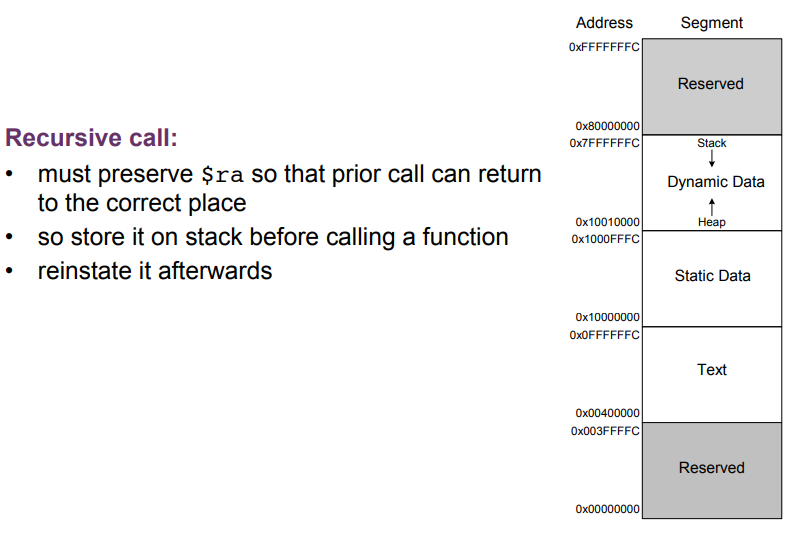
\includegraphics[scale=0.7]{Conventions2}\\
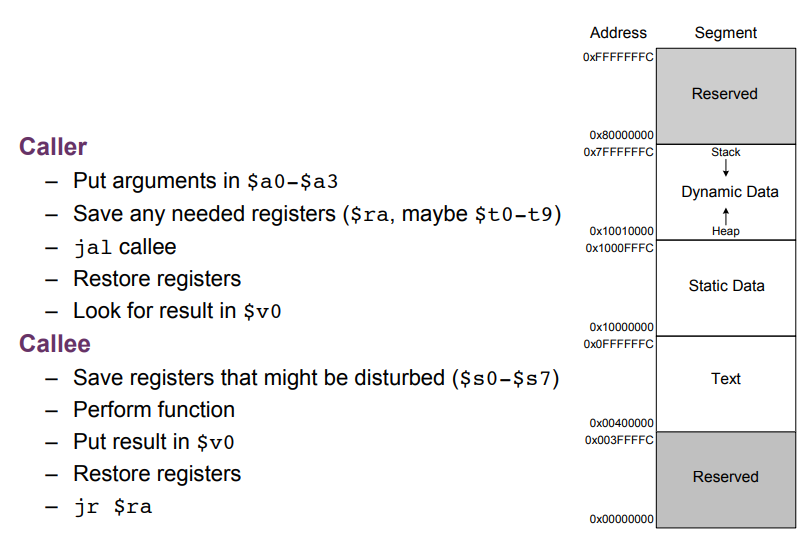
\includegraphics[scale=0.7]{Conventions3}
\section{Example - Factorials}
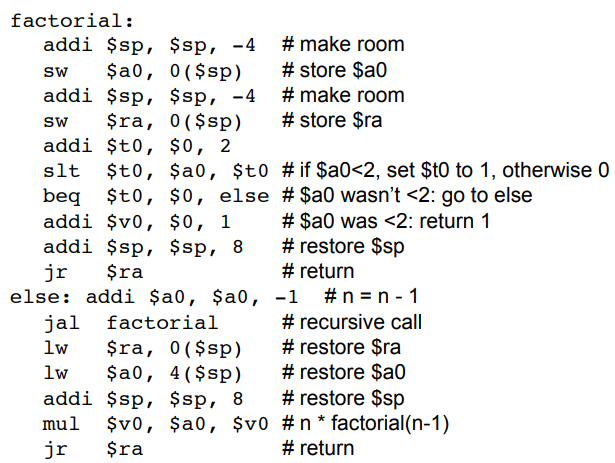
\includegraphics[scale=0.7]{Example}



\end{document}